\chapter{Introduction}	
Nowadays devices are becoming more complex. They embed several subsystems with different characteristics that communicate and interact in many ways. For example, cars can integrate an adaptive control cruise system, GPS tracking, fuel control system and so on. Furthermore, these subsystems are widely coupled. For instance, the adaptive cruise system determines the way to get home depending on the GPS tacking, also, the fuel control system regulates the speed of the car depending on the level of fuel. This makes the design of these systems very complex. A designer has to deal with the heterogeneity of each subsystem but also with the interactions among them. To deal with this inherent complexity, the design is split into different domains, \eg mechanical, electronic, software. The development is thus talcked by different \emph{Domains Experts}.

Model Driven Engineering (MDE) promotes the use of Domain Specific Modeling Languages (DSMLs) to model complex systems using the adequate, domain-specific, terminology and tools (see Figure~\ref{ch:background}). DSMLs are developed by \emph{Language Engineers}\footnote{Also called Domain Experts.} as dedicated languages to make a description of a domain relying on the expert terminology so at to reduce introducing discrepancies in the model. Models must include structural aspects but also behavioral ones. Thus defining a DSML consists in defining its syntax but also its behavioral semantics. When several DSMLs, with different syntax and or semantics, are used conjointly to model a complex system, we say the model is \emph{heterogeneous}, \ie it is made of models that conform to different languages. Dealing with this kind of heterogeneity is the problem addressed in this thesis. 

With heterogeneous models, the overall behavior emerges from its parts. To perform verification and validation activities of the whole system, designers need tools to comprehend this emerging behavior, 
or at least some aspects of it depending on the domain of interest. It is therefore necessary to specify how models and languages are related to each other, in both a structural and a behavioral way.

In this context, the GEMOC initiative proposes to coordinate and disseminate the research results regarding the support of the coordinated use of various modeling languages, that is, the use of multiple modeling languages to support heterogeneous development of diverse aspects of a system. This thesis is part of GEMOC project and it focuses on the coordination~\cite{coordsignibib} of behavioral models to provide simulation and/or verification capabilities for the whole system specification. 


\begin{figure}
	\begin{center}
		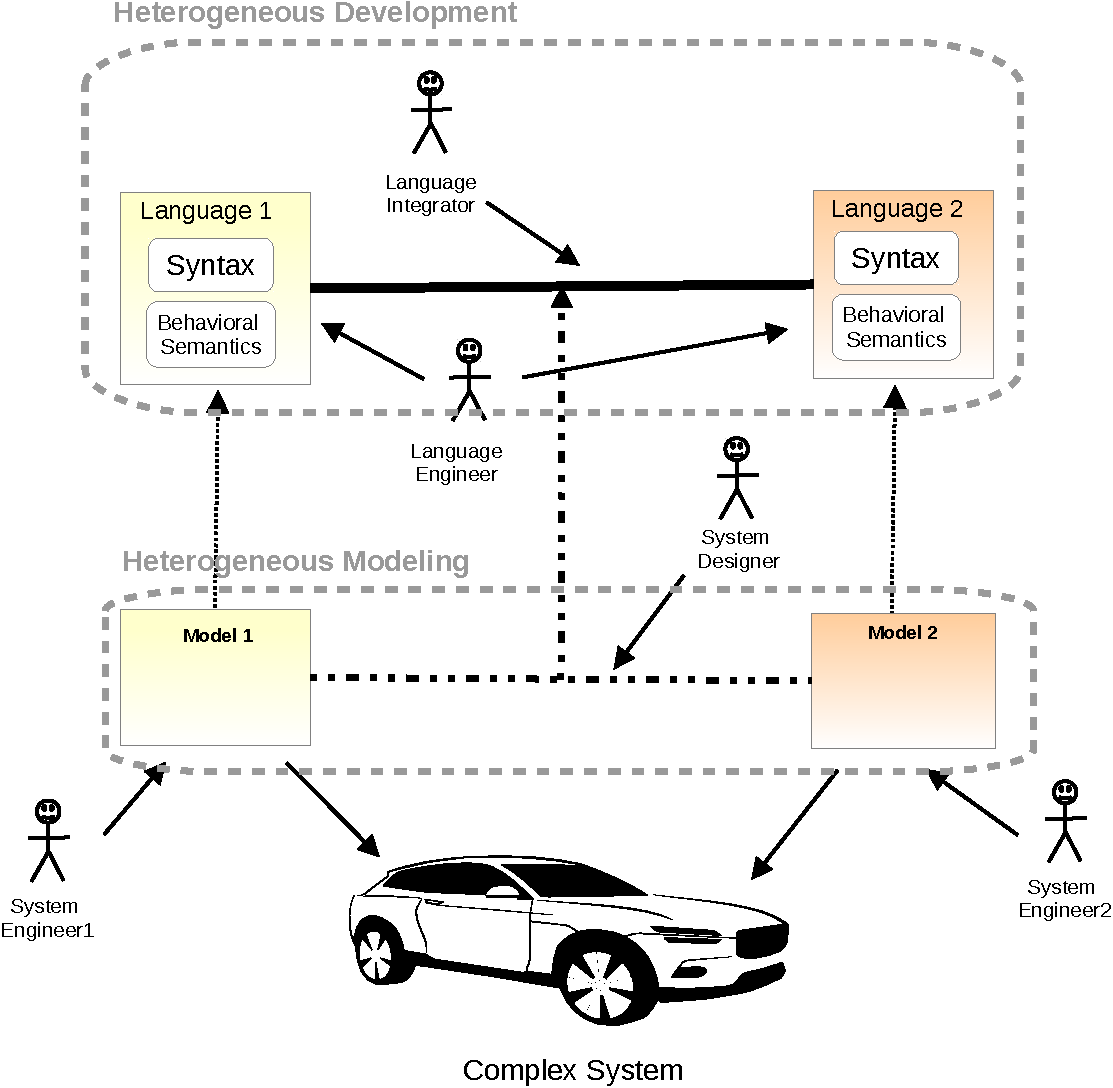
\includegraphics[width=1\textwidth]{introduction/stakeholders}
		\caption{Stakeholders in the development of a Complex System}
		\label{fig:stackeholders}
	\end{center}
\end{figure}
	
Currently, Coordination Languages~\cite{coordsignibib} and Architecture Description Languages (ADLs)~\cite{frameadlsbib} provide dedicated languages to specify the coordination between particular behavioral models. This is usually done by system designers that apply some coordination patterns according to their own skills and know-how. However, in large heterogeneous systems, the manual coordination of models can become tedious and error prone. To automate this task, Coordination frameworks~\cite{ptoleframebib,modhelxbib} have encoded a predefined coordination pattern inside a tool. However, the customization of these tools for a specific domain is difficult. Moreover, these approaches rely on a general purpose language (GPL) to express the coordination thus limiting reasoning about how a system is coordinated.  
	
In this thesis, we deal with the coordination of heterogeneous behavioral models by leveraging on the system designer's skills. We propose a dedicated language named \bcool (standing for \emph{B}ehavioral \emph{C}oordination \emph{O}perat\emph{o}r \emph{L}anguage) that allows for capturing coordination patterns between a given set of DSMLs. These patterns are specified at language level, and then used to derive a coordination model automatically for models conforming to the targeted DSMLs. The coordination at the language level relies on a so-called \emph{language behavioral interface}. This interface exposes an abstraction of the language behavioral semantics in terms of Events. Thus, a \emph{Language Integrator} uses \bcool to define operators that specify how events from different language behavioral interfaces interact. These operators are defined at the language level but they are applied between models to coordinate their behavior. This results in a model of coordination in \ccsl, a declarative language that describes causal and temporal relationships between events. By relying on \ccsl, we provide verification and validation facilities for the coordinated system. All this has been implemented as a set of plugins for Eclipse as part of the GEMOC studio\footnote{http://www.gemoc.org/studio}; which integrates technologies based on Eclipse Modeling Framework (EMF)~\footnote{http://eclipse.org/modeling/emf/} adequate for the specification of executable domain specific modeling languages. %\todo{In the studio, \bcool provides coordination facilities.}   

We organize the content of this thesis in six chapters. Chapter~\ref{ch:background} presents the state-of-art approaches that addressed the problem of getting a global representation of a heterogeneous system, \ie a system that is developed by using different DSMLs. We categorize the background into approaches that \emph{compose} models/languages and approaches that \emph{coordinate} models/languages. In this thesis, we focus on the latter, more precisely, in approaches that specify coordination patterns between languages to automate the coordination between models.  

Chapter~\ref{ch:framework} presents the requirements for a language to specify coordination patterns. We first present a framework to characterize coordination pattern approaches. Then, we use this framework to compare exiting approaches. From this comparison, we state the requirements to make existing approaches more flexible/well founded. Based on these requirements, we propose a particular implementation of the framework, \ie \bcool. 

Chapter~\ref{ch:bcool} presents the implementation of \bcool. We rely on a running example: the coordination of the heterogeneous model of a coffee machine, which is built by using timed finite state machines and activity diagrams. Then, we use this example through all the chapter to illustrate the syntax and semantics of \bcool. We present the current implementation in the GEMOC studio by executing and verifying the coffee machine models. 

To validate our approach, we present in chapter~\ref{ch:examples} the heterogeneous model of a surveillance video system decomposed into three sub-systems. To coordinate these sub-systems, we propose a set of \bcool operators that capture the specification of hierarchical coordination patterns. We use this example as a use case to illustrate the different steps from the specification of the coordination patterns, the coordination of a particular model and the verification of the coordinated system.     

Finally, we provide the conclusion of this work, highlighting its main contributions and we give some perspectives in chapter~\ref{ch:conclusions}.

%\item Section~\ref{sec:coord-lang} presents the main issues in the coordination of behavioral models, and shows how they can be tackled by explicitly capturing coordination patterns at the language level. Section~\ref{sec:interfaceandexample} defines the notion of language behavioral interface by using an example language named Timed Finite State Machine (TFSM). This language is used later in Section~\ref{sec:BCOol} to illustrate \bcool. In Section~\ref{sec:caseStudies}, we validate the approach by using \bcool to capture three coordination patterns between two languages: TFSM and fUML Activities. Section~\ref{sec:related} gives an overview and comparison to related work. Section~\ref{sec:conclu} concludes with a brief summary and a discussion of ongoing and future actions.
	
%\item Finally, we provide the conclusion of this work, highlighting its main contributions and we give some future perspectives in Chapter 7.
	


%\begin{landscape}
%\begin{figure}
%	\begin{center}
%		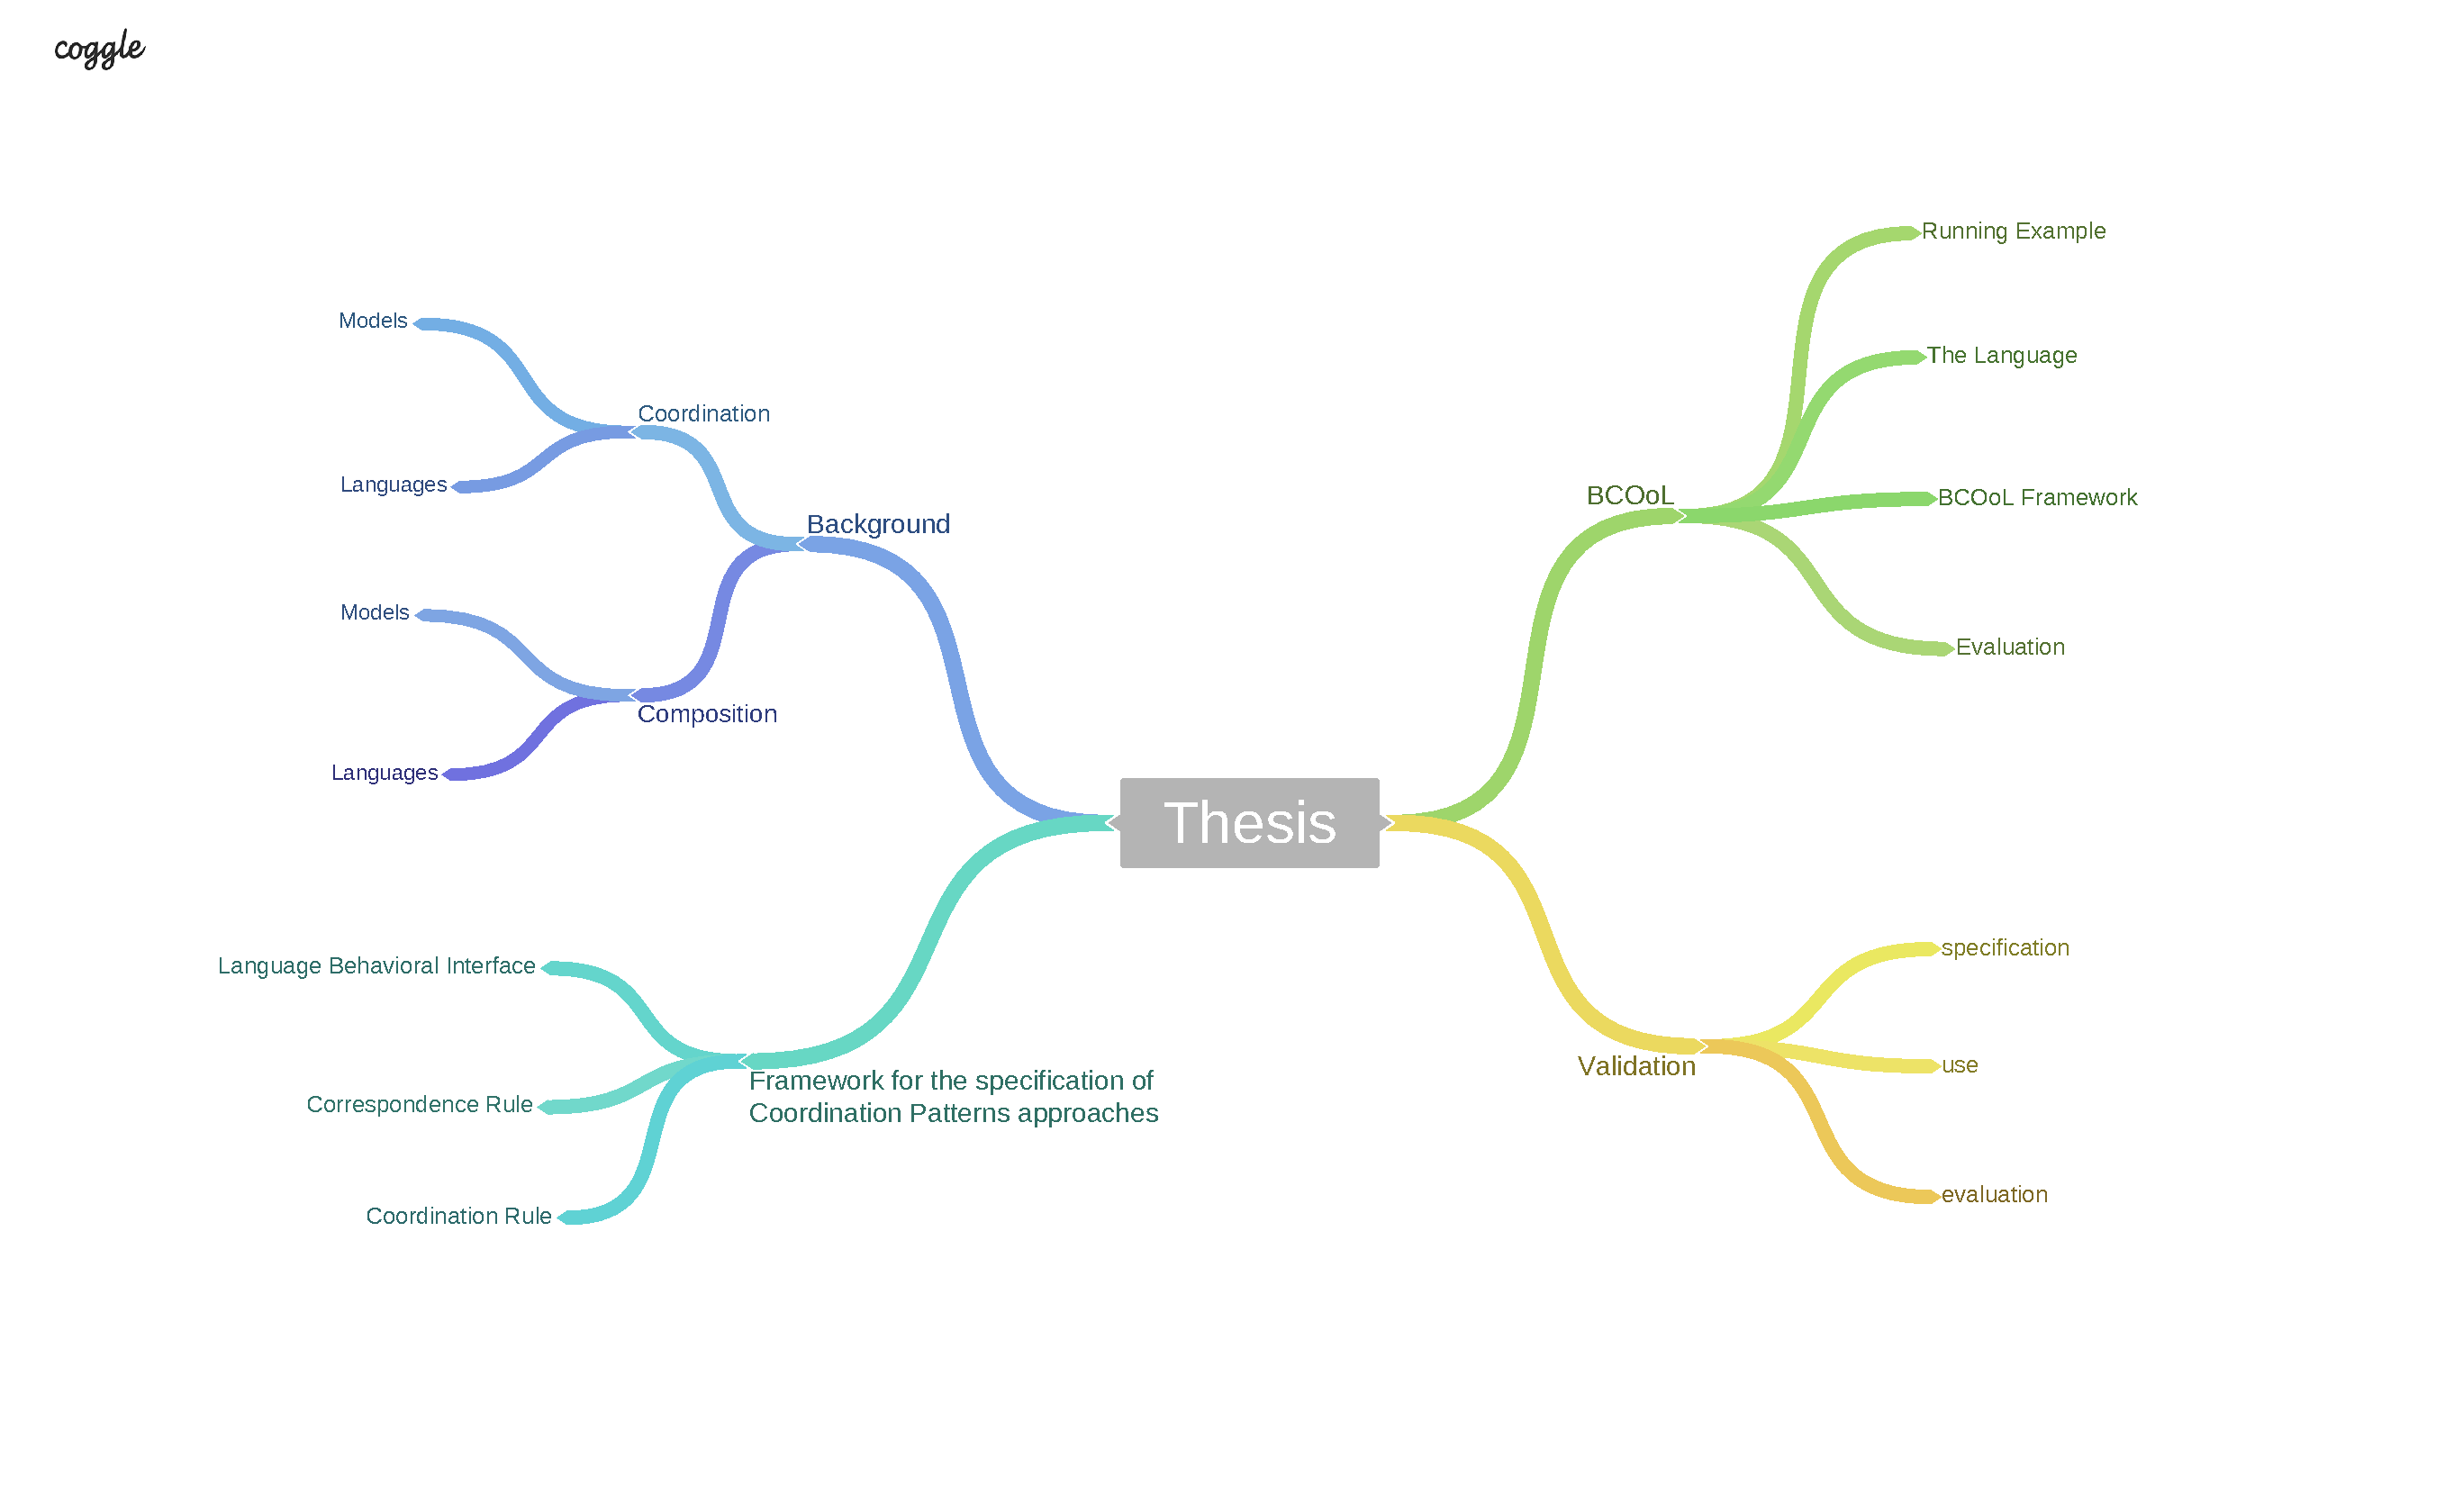
\includegraphics[width=1\textwidth]{Thesisoutline.pdf}
%		\label{fig:thesis outline}
%	\end{center}
%\end{figure}
%\end{landscape}

%\section{Problem}

%\section{Contributions}

%Contributions here.

%\section{Publications}

%Publications here.